\chapter{Oil, Gas, and the Structure of Industrial Wealth}

These notes, drawn from a School of Hard Knocks interview and curated by LazyingArt LLC, follow a field-level investigation of oil and gas as a machine for creating wealth. The lecture does not begin with a balance sheet or a legal chart. It begins with a provocation: oil and gas may have created more durable fortunes than the glamorous sectors that dominate public attention. From there we are taken to the field, to the rig, to the control room, and only then to the deeper structure underneath the industry: distressed asset purchases, day-rate economics, monitoring systems, lease terms, royalty claims, and the split between mineral ownership and working-interest exposure. We will keep that order, because the explanation depends on it.

\section{The Hidden Wealth Machine in the Field}

The lecture opens with a large claim and then immediately narrows it to a place. Oil and gas is introduced not merely as a commodity sector, but as an industry that has built dynasties, powered nations, and continued to mint very large fortunes even while public attention moves elsewhere. Then the rhetoric contracts. We are no longer speaking about civilization in the abstract; we are in El Campo, Texas, in the middle of nowhere, standing near a live rig.

That movement matters. The host's promise is not just that oil is big, but that we can examine the machinery of the business from the ground up. Why does this industry make people rich? Why is it obscure to ordinary investors? Why does it look, from the outside, like a relic, and from the inside, like a continuing engine of wealth? These are the questions that structure the rest of the chapter.

One should notice, even at the outset, that the lecture treats oil and gas less as a single market than as a layered system. There is the physical layer of rigs, wells, pipe, and monitoring. There is the legal layer of leases, royalty interests, and mineral title. And there is the financial layer of capital raising, distressed acquisition, and investor participation. The central interest of the lecture lies in how these layers are tied together.

\section{From Roughneck Labor to an Integrated Business}

Brent Franklin's origin story arrives early because the lecture wants to remove some of the mystique from entry into the field. He did not begin as a polished financier. He describes himself as mowing grass after leaving the Navy, receiving a call from a friend in Midland--Odessa, taking a job on an oil rig, and then, a few years later, buying rigs of his own. The biographical point is not sentimentality. It is structural. In this industry, knowledge is tied to machinery, risk, and repetitive exposure to the physical work.

The lecture then supplies scale. Brent says that the company did about
\begin{equation}
R_{\mathrm{year}} \approx 40 \times 10^6\ \mathrm{USD}
\end{equation}
in the last year across all of its platforms. The important phrase is \emph{across all of its platforms}. He does not present the business as a single lucky well. He presents it as an integrated stack: buying distressed off-market oil and gas properties, fixing them, drilling wells, fixing wells, and building a fund structure through which investors can participate without themselves becoming operators.

This is the first genuinely economic clarification of the lecture. From a distance, one imagines ``oil wealth'' as a gush of commodity revenue. At field level, however, the business is more interesting. It can include service income, asset acquisition, operational turnaround, lease economics, and capital structuring. The glamour of the commodity sits on top of a less glamorous but more intelligible arrangement of machines and contracts.

\begin{table}[h]
\centering
\begin{tabular}{|l|l|}
\hline
Quantity & Value reported in the lecture \\
\hline
Annual business scale & \(R_{\mathrm{year}} \approx 40 \times 10^6\ \mathrm{USD}\) \\
Rig day rate & \(R_{\mathrm{day}} = 15{,}500\ \mathrm{USD/day}\) \\
Replacement cost of rig & \(C_{\mathrm{new}} \approx 6.5 \times 10^6\ \mathrm{USD}\) \\
Purchase basis & about \(15\%\) of replacement cost \\
Whole depth on monitor & \(D = 4599.5\ \mathrm{ft}\) \\
Starter capital benchmark & \(K_0 \approx \$100{,}000\) \\
Rig specification & top-drive rig, about \(850\) horsepower \\
\hline
\end{tabular}
\caption{Quantitative markers carried explicitly by the interview.}
\end{table}

The arithmetic of distressed acquisition is one of the cleanest pieces of mathematics in the lecture. Brent says that a brand-new version of the rig on site would cost about
\begin{equation}
C_{\mathrm{new}} \approx 6.5 \times 10^6\ \mathrm{USD},
\end{equation}
while his company bought the actual rig for about fifteen cents on the dollar:
\begin{equation}
C_{\mathrm{buy}} \approx 0.15\,C_{\mathrm{new}} \approx 0.15 \times 6.5 \times 10^6 \approx 9.75 \times 10^5\ \mathrm{USD}.
\end{equation}
He adds that the prior owner had paid over five million dollars for the same equipment. The point is not merely that bankruptcy creates bargains. It is that industrial wealth can begin with replacement-cost asymmetry: if one can buy service equipment far below new-build cost, then the operating business sits on a radically different basis than the business of a buyer who paid full freight.

\paragraph{Worked example.} The acquisition logic can be written in four simple steps:
\begin{enumerate}
\item Start from the reported replacement benchmark \(C_{\mathrm{new}} \approx 6.5 \times 10^6\ \mathrm{USD}\).
\item Apply the stated distressed discount \(C_{\mathrm{buy}} \approx 0.15\,C_{\mathrm{new}}\).
\item Compute the implied purchase basis:
\[
C_{\mathrm{buy}} \approx 9.75 \times 10^5\ \mathrm{USD}.
\]
\item Interpret the spread not as paper profit, but as room to operate a real machine under inherited contracts and day-rate monetization.
\end{enumerate}

Already we see the lecture's first serious theme. Oil wealth is not only about what comes out of the ground. It is also about when assets are bought, from whom, and under what stress.

\section{Why Oil Makes Fortunes and Eats Fortunes}

Immediately after the wealth claim comes the correction. Brent gives the old line: if one wants to make a small fortune in oil and gas, one should start with a large fortune. That is not an afterthought. It is the first attempt to distinguish romantic talk from operating truth.

The lecture insists on three conditions: consistency, diversification, and risk tolerance. This is the first place where the notes should slow down. Oil and gas is not presented as a lottery ticket. It is presented as a field in which fortunes are made by surviving volatility, buying well, structuring correctly, and not concentrating all one's exposure in a single fragile bet.

\subsection{Question \& Answer}

\paragraph{Question.} If oil and gas makes people rich, why do so many people lose money in it?

\paragraph{Answer.} Because the lecture's notion of wealth here is structural rather than magical. A single well can fail. A promoter can overstate the opportunity. A property can be overleveraged. An investor can misunderstand the legal form of the deal. And a technically sound project can still produce poor results if capital is concentrated in the wrong place at the wrong time. The lecture therefore distinguishes, quite sharply, between \emph{participating in the upside} and \emph{surviving the downside}.

This distinction appears again when Brent advises that even a serious initial amount of capital should not be placed all at once into one well, one new drill, or one company. If we let the outsider's starting capital be
\begin{equation}
K_0 \approx \$100{,}000,
\end{equation}
then the discipline he recommends is not
\[
K_1 = K_0
\]
for a single exposure, but rather a partition,
\begin{equation}
K_0 = \sum_{i=1}^{n} K_i,
\end{equation}
across multiple wells, operators, or deal structures. The lecture's language is careful here: there may be no way to abolish risk, but there may be a way to mitigate loss.

The broader lesson is that oil and gas punishes conceptual laziness. One must know what one owns, what one is paid for, what losses one is exposed to, and how much operational competence stands behind the offering. Only after that can the industry be discussed as a wealth machine.

\section{The Rig as a 24/7 Business Machine}

The lecture next descends from capital language into operational language. We are shown the camp house, introduced to the tool pusher, and told that drilling is a \(24\)-hour operation. The claim is not decorative. It means that the business cannot be understood as the work of a lone proprietor. It requires a team, indeed what Brent calls an army: experienced people, shift continuity, safety discipline, and a constant interpretation of what the equipment is doing.

This operational emphasis is reinforced by the safety discussion. The lecture points to fire-retardant clothing, heavy moving parts, sharp objects, and the danger of live industrial equipment. It also notes the importance of H\(_2\)S monitoring on sites where that gas may be present. Here the lecture performs one of its most useful conceptual reversals: the public sees ``black gold and money,'' but the operator sees heavy loads, exposure, and the need for procedural control.

The doghouse is the first place where the lecture becomes almost mathematical in the narrow sense. Brent points to the monitoring system and explains that it functions as the rig's electronic eyes and ears. It tells the crew the whole depth of the hole, where the bit is, what operation is currently underway, and what formations or gas signatures are being encountered. In the lecture's reported state, the whole depth is
\begin{equation}
D = 4599.5\ \mathrm{ft},
\end{equation}
and the current state is ``tripping,'' which we may write in cautious standard notation as
\begin{equation}
s \in \{\text{drilling},\ \text{tripping in},\ \text{tripping out}\}, \qquad s=\text{tripping}.
\end{equation}
Here ``tripping'' means moving pipe in or out of the hole by adding or removing joints rather than cutting fresh depth. The monitor therefore does not merely display numbers. It translates hidden mechanical action into an interpretable operational state.

\begin{figure}[h]
\centering
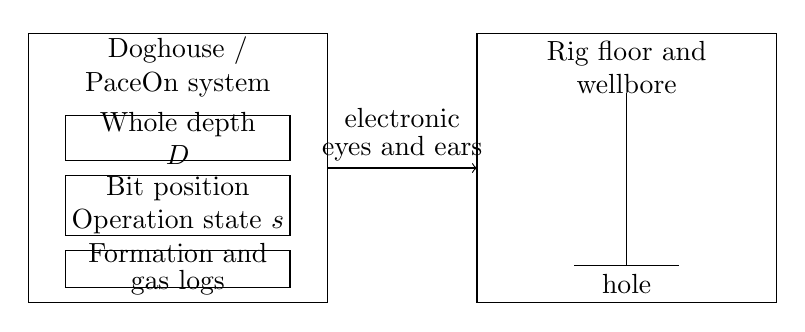
\begin{tikzpicture}[scale=0.95]
\draw (-5,1.8) rectangle (-1,-1.8);
\node at (-3,1.35) {\shortstack{Doghouse /\\PaceOn system}};
\draw (-4.5,0.7) rectangle (-1.5,0.1);
\node at (-3,0.4) {\shortstack{Whole depth\\\(D\)}};
\draw (-4.5,-0.1) rectangle (-1.5,-0.9);
\node at (-3,-0.5) {\shortstack{Bit position\\Operation state \(s\)}};
\draw (-4.5,-1.1) rectangle (-1.5,-1.6);
\node at (-3,-1.35) {\shortstack{Formation and\\gas logs}};

\draw (1,1.8) rectangle (5,-1.8);
\node at (3,1.35) {\shortstack{Rig floor and\\wellbore}};
\draw (3,1.0) -- (3,-1.3);
\draw (2.3,-1.3) -- (3.7,-1.3);
\node at (3,-1.55) {hole};

\draw[->] (-1,0) -- (1,0);
\node at (0,0.45) {\shortstack{electronic\\eyes and ears}};
\end{tikzpicture}
\caption{Transcript-derived schematic of the operational picture. The floor itself is noisy and partially opaque; the doghouse converts activity in the hole into depth, bit position, state, and formation information.}
\end{figure}

\subsection{Question \& Answer}

\paragraph{Question.} If we cannot see into the well, what exactly does the driller know?

\paragraph{Answer.} The driller knows the hole indirectly but continuously. He does not see the subsurface as one sees a room. He sees a state vector assembled from instruments: total depth, the bit's position, whether the crew is drilling or tripping, and the logs that report the character of the formation. The lecture's claim is not that technology removes danger; it is that modern drilling is no longer blind in the way it once was.

After a brief interruption in the video, the lecture returns to the rig and performs another necessary clarification: a rig is not a well. The rig is the machine that drills; the well is the asset thereby created.

\begin{definition}
In the language of the lecture, a \emph{drilling rig} is the service machine that drills or services the hole, while a \emph{well} is the drilled asset itself. Owning the former is exposure to day-rate service income; owning the latter is exposure to production and the legal structure of the lease.
\end{definition}

This distinction matters because the rig on site is explicitly described as an \(850\)-horsepower top-drive drilling rig, and its economics are not initially the economics of production. They are the economics of service:
\begin{equation}
R_{\mathrm{day}} = 15{,}500\ \mathrm{USD/day}.
\end{equation}
If one writes a ceiling-style annualization with utilization \(u \in [0,1]\), one obtains
\begin{equation}
R_{\mathrm{rig,annual}} = 365\,u\,R_{\mathrm{day}}.
\end{equation}
This is not a claim about realized yearly income for this particular rig. It is simply the bookkeeping relation that the lecture wants us to notice: a machine bought below replacement cost can be monetized by daily operation under contract.

\section{How an Outsider Is Allowed to Invest}

Only after the lecture has shown us machinery, safety, and monitoring does it return to the outsider's question: how does one get in? Brent's answer is restrictive rather than democratic. In the lecture's language, oil and gas investments are ordinarily structured for accredited investors; elsewhere he also uses the phrase ``licensed investor.'' The economically relevant point is clear even if the legal vocabulary is loose: this is not being presented as a casual retail market.

The lecture gives three filters. First, one must meet the relevant investor gate. Second, one must have substantial capital. Third, and most importantly, one must be able to bear total loss before entering the field. The benchmark offered in the lecture is
\begin{equation}
K_0 \approx \$100{,}000,
\end{equation}
but even this is not described as a sum to be placed all at once into one hole in the ground. The warning against concentration is emphatic.

This is also where the lecture presents the investment sales pitch in its strongest form. Brent argues that people are drawn to oil and gas for tax treatment and for unusually high upside when deals are structured properly. He contrasts this with real estate, which he praises for long-term appreciation, and with the stock market, which he describes as a place where unsophisticated investors often ride waves they do not understand. His own conclusion is not the abolition of other markets, but diversification across them.

\begin{remark}
The lecture presents two strong claims here: first, that properly structured oil-and-gas investments may provide tax advantages against active income; second, that some deals can return more than \(100\%\) in less than a year. We record these as attributed claims about structure and operator quality, not as general guarantees of the asset class.
\end{remark}

In the lecture's compressed notation, one may summarize that claim as
\begin{equation}
\mathrm{ROI} > 100\%, \qquad t < 1\ \mathrm{year},
\end{equation}
but the surrounding prose matters more than the inequality. Brent's point is that these outcomes belong, if at all, to correctly structured deals run by competent operators and purchased with proper risk tolerance. The inequality by itself is not a theorem.

\section{Rig, Well, Lease, Royalty, Working Interest}

This is the deepest and most useful section of the lecture. After discussing investing in general, Brent shifts to the structure of the industry itself. First comes the three-part chain:
\begin{equation}
\text{upstream} \longrightarrow \text{midstream} \longrightarrow \text{downstream}.
\end{equation}
Upstream refers to drilling and extraction. Midstream refers to movement, shipping, and transport. Downstream refers to refining and finished products. This matters because the lecture explicitly corrects the naive idea that the operator simply ``sells gasoline.'' The path from hole to end product runs through several distinct businesses.

Then comes the legal split that most outsiders do not see. The person who owns the land at the surface need not own the minerals beneath it. There may be one mineral owner; there may be many. The landman enters at precisely this point, identifying title, assembling the relevant interests, and negotiating the oil-and-gas lease.

From there we arrive at the lecture's main payout logic. Let \(G\) denote gross production revenue. If the royalty rate is
\begin{equation}
r = 25\% = 0.25,
\end{equation}
then the lecture's practical split is
\begin{align}
G &= rG + (1-r)G, \\
  &= 0.25\,G + 0.75\,G.
\end{align}
The mineral-owner side receives the royalty share before expenses. The operator side receives the remainder. In the lecture's practical vocabulary, this mineral-owner gross share is also discussed through the label NRI. Thus if one is told that
\begin{equation}
\mathrm{NRI} = 20\% = 0.20,
\end{equation}
the lecture wants us to read
\begin{equation}
G = 0.20\,G + 0.80\,G,
\end{equation}
with the \(20\%\) going to the mineral-owner side and the \(80\%\) remaining on the operator side.

That remainder is then identified as the working-interest side, the side that actually bears drilling and operating costs. A cautious standard reconstruction is therefore
\begin{equation}
\Pi_{\mathrm{WI}} = (1-r)G - C_{\mathrm{drill}} - C_{\mathrm{op}},
\end{equation}
and if an investor purchases a fraction \(\alpha\) of that exposure, then
\begin{equation}
\Pi_{\alpha} = \alpha\,\Pi_{\mathrm{WI}} = \alpha\big((1-r)G - C_{\mathrm{drill}} - C_{\mathrm{op}}\big).
\end{equation}
This is not a line that Brent writes on screen, but it is the cleanest standard form of the mechanism he describes in words: the investor pays into drilling and receives a fraction of the proceeds if the well is commercially productive.

\begin{figure}[h]
\centering
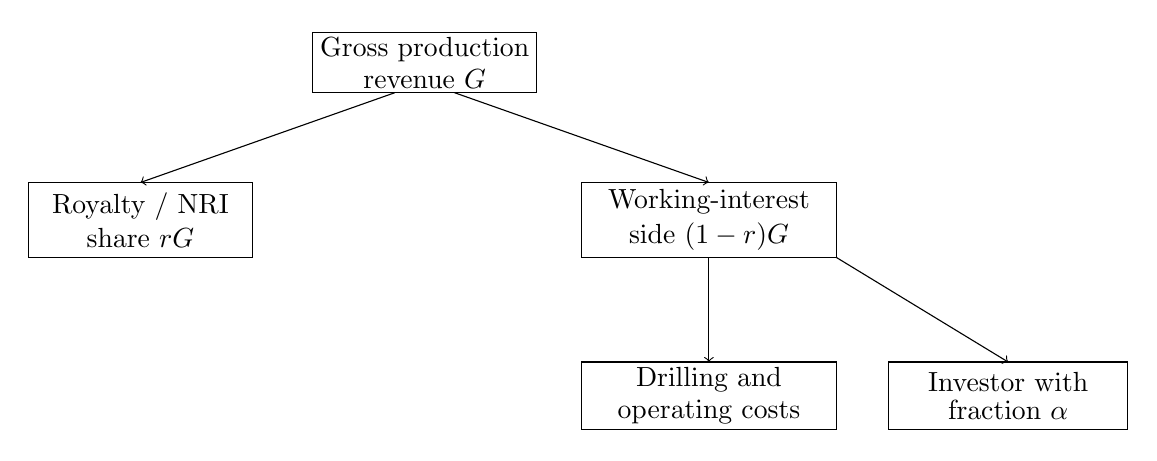
\begin{tikzpicture}[scale=0.95]
\draw (-1.4,3.0) rectangle (1.6,2.2);
\node at (0.1,2.6) {\shortstack{Gross production\\revenue \(G\)}};

\draw (-5.2,1.0) rectangle (-2.2,0.0);
\node at (-3.7,0.5) {\shortstack{Royalty / NRI\\share \(rG\)}};

\draw (2.2,1.0) rectangle (5.6,0.0);
\node at (3.9,0.5) {\shortstack{Working-interest\\side \((1-r)G\)}};

\draw[->] (-0.3,2.2) -- (-3.7,1.0);
\draw[->] (0.5,2.2) -- (3.9,1.0);

\draw (2.2,-1.4) rectangle (5.6,-2.3);
\node at (3.9,-1.85) {\shortstack{Drilling and\\operating costs}};

\draw (6.3,-1.4) rectangle (9.5,-2.3);
\node at (7.9,-1.85) {\shortstack{Investor with\\fraction \(\alpha\)}};

\draw[->] (3.9,0.0) -- (3.9,-1.4);
\draw[->] (5.6,0.0) -- (7.9,-1.4);
\end{tikzpicture}
\caption{Transcript-derived revenue and exposure schematic. In the lecture's practical presentation, gross revenue first splits between the mineral-owner share and the working-interest side; costs live on the working-interest side.}
\end{figure}

\subsection{Question \& Answer}

\paragraph{Question.} Who owns what, and who gets paid first when oil and gas is produced?

\paragraph{Answer.} The lecture's answer is layered. Surface ownership and mineral ownership may be different. The operator typically enters through a lease assembled by title work and negotiation. Once production exists, the mineral-owner share is carved out of gross proceeds first through the royalty or NRI language of the lease. The working-interest side receives what remains and is the side against which the costs of drilling and operation are charged. That is why the same well can look safe from one side and risky from another: the sides are not economically identical.

\begin{table}[h]
\centering
\begin{tabular}{|l|p{8.5cm}|}
\hline
Term & Practical meaning in the lecture \\
\hline
Surface owner & Owns the land at the surface level. \\
Mineral owner & Owns the subsurface mineral estate; may be one person or many. \\
Landman & Identifies title, assembles the area of interest, and negotiates leases. \\
Royalty & Share of gross proceeds paid before expenses to the mineral-owner side. \\
NRI & In the lecture's language, the mineral-owner gross share of revenue. \\
Working interest & The remaining side of the deal; exposed to drilling and operating costs as well as upside. \\
Rig & The service machine that drills. \\
Well & The drilled asset from which production may later flow. \\
\hline
\end{tabular}
\caption{Terms as they function in the interview. Petroleum-law usage is more technical, but this is the operational vocabulary of the lecture.}
\end{table}

At this point the lecture has largely completed its mathematical payload. We know how the speaker thinks the industry is divided, how a service machine can become a revenue source, how production revenue is split, and why the outsider cannot understand the industry without separating physical equipment, legal title, and capital structure.

\section{Natural Gas, Marketing, and the Operator's Philosophy}

The closing movement of the lecture turns outward again. Brent says that his present focus is not oil but natural gas exploration and production. Oil, in his description, involves additional mechanical frustrations: pump jacks, failures, and the burdens of mature production equipment. Natural gas, by contrast, is presented as the cleaner-burning fossil fuel and as the commodity better positioned for current demand growth through LNG export, electricity generation, heating, data centers, and even Bitcoin mining fed by gas-powered generation.

This shift matters because it preserves the lecture's recurring motif of neglected opportunity. The industry is old, but the opportunity is not simply old. It can be renewed by a change in demand, by a neglected sub-sector, or by new ways of converting energy into revenue.

The chapter then broadens one last time into commercial method. Brent argues that marketing is more important than most operators admit, especially in a traditional industry that has not fully absorbed social media and direct audience-building. He contrasts sales and marketing with a memorable asymmetry: one may make millions in sales, but far more in marketing. Beneath the slogan lies a principle that has quietly governed the lecture from the beginning: money does not come from chasing money; it comes from solving problems and monetizing the solution.

This is also why the lecture spends so much time on operator philosophy. The business is not merely rigs, wells, and leases. It is the ability to see a distressed asset where others see wreckage, to see title complexity where others see land, to see monitored state where others see noise, and to build a structure in which capital, operation, and legal rights are aligned. The final claims about doubt, wrong partners, wrong relationships, and the need for results should be read in that light. They are not separate from the economics. They are the speaker's account of what kind of person can inhabit those economics successfully.

\section{Summary}

The lecture begins with a boast about a trillion-dollar industry and ends with a practical map of how that industry is actually organized. The main lesson is that oil and gas wealth is not a single thing. It is a compound of discounted asset purchase, day-rate service income, monitored industrial operation, restrictive investment entry, and legal rights to production revenue. A rig is not a well; a surface owner is not necessarily a mineral owner; gross revenue is not the same thing as working-interest profit. Once these distinctions are made, the industry becomes less mysterious and more severe. It remains dangerous, capital-intensive, and highly unequal in competence. But it also becomes legible. And in this lecture, that legibility is the real beginning of economic understanding.